\documentclass[tikz,border=4pt,11pt]{standalone}
\usepackage{amsmath}
\definecolor{ink}{RGB}{42,52,64}
\definecolor{first}{RGB}{146,79,26}
\definecolor{second}{RGB}{26,99,111}

% The Foata--Strehl (valley-hopping) orbit of 1234 in S_4, with
% sigma_0 = sigma_5 = infinity (dashed ends).  Each permutation is drawn as a
% mountain: the point (i, sigma_i) for i = 1..4.  Double ascents are teal,
% double descents brown, the valley 1 is dark.  Columns are sorted by the
% number of descents (1, 3, 3, 1 permutations), and an edge labelled
% phi_j joins two permutations that differ by the hop of the value j,
% from a double ascent (left) to a double descent (right).  The descent
% polynomial of the orbit is 1+3x+3x^2+x^3 = (1+x)^3; the monomial below each
% column records its permutations.  No legend: the page text explains the
% colours.

\begin{document}
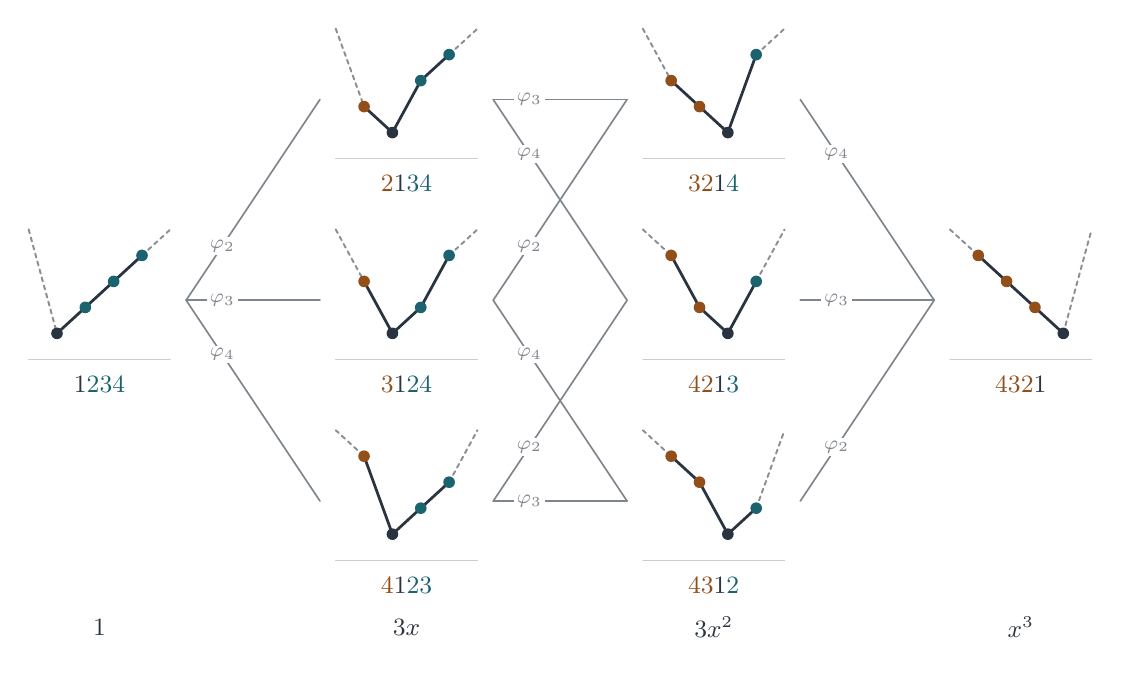
\begin{tikzpicture}[text=ink,line cap=round,line join=round]
  % 1234: des 0
  \begin{scope}[shift={(0.00,0.00)}]
    \draw[ink!25,line width=.4pt] (0,0) -- (1.80,0);
    \draw[ink!55,line width=.7pt,dash pattern=on 1.5pt off 1.5pt] (0,1.65) -- (0.36,0.33);
    \draw[ink!55,line width=.7pt,dash pattern=on 1.5pt off 1.5pt] (1.44,1.32) -- (1.80,1.65);
    \draw[ink,line width=1pt] (0.36,0.33) -- (0.72,0.66) -- (1.08,0.99) -- (1.44,1.32);
    \fill[ink] (0.36,0.33) circle (2.1pt);
    \fill[second] (0.72,0.66) circle (2.1pt);
    \fill[second] (1.08,0.99) circle (2.1pt);
    \fill[second] (1.44,1.32) circle (2.1pt);
    \node[font=\small] at (0.90,-.32) {$\textcolor{ink}{1}\textcolor{second}{2}\textcolor{second}{3}\textcolor{second}{4}$};
  \end{scope}
  % 2134: des 1
  \begin{scope}[shift={(3.90,2.55)}]
    \draw[ink!25,line width=.4pt] (0,0) -- (1.80,0);
    \draw[ink!55,line width=.7pt,dash pattern=on 1.5pt off 1.5pt] (0,1.65) -- (0.36,0.66);
    \draw[ink!55,line width=.7pt,dash pattern=on 1.5pt off 1.5pt] (1.44,1.32) -- (1.80,1.65);
    \draw[ink,line width=1pt] (0.36,0.66) -- (0.72,0.33) -- (1.08,0.99) -- (1.44,1.32);
    \fill[first] (0.36,0.66) circle (2.1pt);
    \fill[ink] (0.72,0.33) circle (2.1pt);
    \fill[second] (1.08,0.99) circle (2.1pt);
    \fill[second] (1.44,1.32) circle (2.1pt);
    \node[font=\small] at (0.90,-.32) {$\textcolor{first}{2}\textcolor{ink}{1}\textcolor{second}{3}\textcolor{second}{4}$};
  \end{scope}
  % 3124: des 1
  \begin{scope}[shift={(3.90,0.00)}]
    \draw[ink!25,line width=.4pt] (0,0) -- (1.80,0);
    \draw[ink!55,line width=.7pt,dash pattern=on 1.5pt off 1.5pt] (0,1.65) -- (0.36,0.99);
    \draw[ink!55,line width=.7pt,dash pattern=on 1.5pt off 1.5pt] (1.44,1.32) -- (1.80,1.65);
    \draw[ink,line width=1pt] (0.36,0.99) -- (0.72,0.33) -- (1.08,0.66) -- (1.44,1.32);
    \fill[first] (0.36,0.99) circle (2.1pt);
    \fill[ink] (0.72,0.33) circle (2.1pt);
    \fill[second] (1.08,0.66) circle (2.1pt);
    \fill[second] (1.44,1.32) circle (2.1pt);
    \node[font=\small] at (0.90,-.32) {$\textcolor{first}{3}\textcolor{ink}{1}\textcolor{second}{2}\textcolor{second}{4}$};
  \end{scope}
  % 4123: des 1
  \begin{scope}[shift={(3.90,-2.55)}]
    \draw[ink!25,line width=.4pt] (0,0) -- (1.80,0);
    \draw[ink!55,line width=.7pt,dash pattern=on 1.5pt off 1.5pt] (0,1.65) -- (0.36,1.32);
    \draw[ink!55,line width=.7pt,dash pattern=on 1.5pt off 1.5pt] (1.44,0.99) -- (1.80,1.65);
    \draw[ink,line width=1pt] (0.36,1.32) -- (0.72,0.33) -- (1.08,0.66) -- (1.44,0.99);
    \fill[first] (0.36,1.32) circle (2.1pt);
    \fill[ink] (0.72,0.33) circle (2.1pt);
    \fill[second] (1.08,0.66) circle (2.1pt);
    \fill[second] (1.44,0.99) circle (2.1pt);
    \node[font=\small] at (0.90,-.32) {$\textcolor{first}{4}\textcolor{ink}{1}\textcolor{second}{2}\textcolor{second}{3}$};
  \end{scope}
  % 3214: des 2
  \begin{scope}[shift={(7.80,2.55)}]
    \draw[ink!25,line width=.4pt] (0,0) -- (1.80,0);
    \draw[ink!55,line width=.7pt,dash pattern=on 1.5pt off 1.5pt] (0,1.65) -- (0.36,0.99);
    \draw[ink!55,line width=.7pt,dash pattern=on 1.5pt off 1.5pt] (1.44,1.32) -- (1.80,1.65);
    \draw[ink,line width=1pt] (0.36,0.99) -- (0.72,0.66) -- (1.08,0.33) -- (1.44,1.32);
    \fill[first] (0.36,0.99) circle (2.1pt);
    \fill[first] (0.72,0.66) circle (2.1pt);
    \fill[ink] (1.08,0.33) circle (2.1pt);
    \fill[second] (1.44,1.32) circle (2.1pt);
    \node[font=\small] at (0.90,-.32) {$\textcolor{first}{3}\textcolor{first}{2}\textcolor{ink}{1}\textcolor{second}{4}$};
  \end{scope}
  % 4213: des 2
  \begin{scope}[shift={(7.80,0.00)}]
    \draw[ink!25,line width=.4pt] (0,0) -- (1.80,0);
    \draw[ink!55,line width=.7pt,dash pattern=on 1.5pt off 1.5pt] (0,1.65) -- (0.36,1.32);
    \draw[ink!55,line width=.7pt,dash pattern=on 1.5pt off 1.5pt] (1.44,0.99) -- (1.80,1.65);
    \draw[ink,line width=1pt] (0.36,1.32) -- (0.72,0.66) -- (1.08,0.33) -- (1.44,0.99);
    \fill[first] (0.36,1.32) circle (2.1pt);
    \fill[first] (0.72,0.66) circle (2.1pt);
    \fill[ink] (1.08,0.33) circle (2.1pt);
    \fill[second] (1.44,0.99) circle (2.1pt);
    \node[font=\small] at (0.90,-.32) {$\textcolor{first}{4}\textcolor{first}{2}\textcolor{ink}{1}\textcolor{second}{3}$};
  \end{scope}
  % 4312: des 2
  \begin{scope}[shift={(7.80,-2.55)}]
    \draw[ink!25,line width=.4pt] (0,0) -- (1.80,0);
    \draw[ink!55,line width=.7pt,dash pattern=on 1.5pt off 1.5pt] (0,1.65) -- (0.36,1.32);
    \draw[ink!55,line width=.7pt,dash pattern=on 1.5pt off 1.5pt] (1.44,0.66) -- (1.80,1.65);
    \draw[ink,line width=1pt] (0.36,1.32) -- (0.72,0.99) -- (1.08,0.33) -- (1.44,0.66);
    \fill[first] (0.36,1.32) circle (2.1pt);
    \fill[first] (0.72,0.99) circle (2.1pt);
    \fill[ink] (1.08,0.33) circle (2.1pt);
    \fill[second] (1.44,0.66) circle (2.1pt);
    \node[font=\small] at (0.90,-.32) {$\textcolor{first}{4}\textcolor{first}{3}\textcolor{ink}{1}\textcolor{second}{2}$};
  \end{scope}
  % 4321: des 3
  \begin{scope}[shift={(11.70,0.00)}]
    \draw[ink!25,line width=.4pt] (0,0) -- (1.80,0);
    \draw[ink!55,line width=.7pt,dash pattern=on 1.5pt off 1.5pt] (0,1.65) -- (0.36,1.32);
    \draw[ink!55,line width=.7pt,dash pattern=on 1.5pt off 1.5pt] (1.44,0.33) -- (1.80,1.65);
    \draw[ink,line width=1pt] (0.36,1.32) -- (0.72,0.99) -- (1.08,0.66) -- (1.44,0.33);
    \fill[first] (0.36,1.32) circle (2.1pt);
    \fill[first] (0.72,0.99) circle (2.1pt);
    \fill[first] (1.08,0.66) circle (2.1pt);
    \fill[ink] (1.44,0.33) circle (2.1pt);
    \node[font=\small] at (0.90,-.32) {$\textcolor{first}{4}\textcolor{first}{3}\textcolor{first}{2}\textcolor{ink}{1}$};
  \end{scope}
  % edges: phi_j moves j from a double ascent to a double descent
  \draw[ink!60,line width=.6pt] (2.00,0.75) -- node[pos=.27,fill=white,inner sep=1pt,font=\scriptsize] {$\varphi_2$} (3.70,3.30);
  \draw[ink!60,line width=.6pt] (2.00,0.75) -- node[pos=.27,fill=white,inner sep=1pt,font=\scriptsize] {$\varphi_3$} (3.70,0.75);
  \draw[ink!60,line width=.6pt] (2.00,0.75) -- node[pos=.27,fill=white,inner sep=1pt,font=\scriptsize] {$\varphi_4$} (3.70,-1.80);
  \draw[ink!60,line width=.6pt] (5.90,3.30) -- node[pos=.27,fill=white,inner sep=1pt,font=\scriptsize] {$\varphi_3$} (7.60,3.30);
  \draw[ink!60,line width=.6pt] (5.90,3.30) -- node[pos=.27,fill=white,inner sep=1pt,font=\scriptsize] {$\varphi_4$} (7.60,0.75);
  \draw[ink!60,line width=.6pt] (5.90,0.75) -- node[pos=.27,fill=white,inner sep=1pt,font=\scriptsize] {$\varphi_2$} (7.60,3.30);
  \draw[ink!60,line width=.6pt] (5.90,0.75) -- node[pos=.27,fill=white,inner sep=1pt,font=\scriptsize] {$\varphi_4$} (7.60,-1.80);
  \draw[ink!60,line width=.6pt] (5.90,-1.80) -- node[pos=.27,fill=white,inner sep=1pt,font=\scriptsize] {$\varphi_2$} (7.60,0.75);
  \draw[ink!60,line width=.6pt] (5.90,-1.80) -- node[pos=.27,fill=white,inner sep=1pt,font=\scriptsize] {$\varphi_3$} (7.60,-1.80);
  \draw[ink!60,line width=.6pt] (9.80,3.30) -- node[pos=.27,fill=white,inner sep=1pt,font=\scriptsize] {$\varphi_4$} (11.50,0.75);
  \draw[ink!60,line width=.6pt] (9.80,0.75) -- node[pos=.27,fill=white,inner sep=1pt,font=\scriptsize] {$\varphi_3$} (11.50,0.75);
  \draw[ink!60,line width=.6pt] (9.80,-1.80) -- node[pos=.27,fill=white,inner sep=1pt,font=\scriptsize] {$\varphi_2$} (11.50,0.75);
  \node[font=\small] at (0.90,-3.40) {$1$};
  \node[font=\small] at (4.80,-3.40) {$3x$};
  \node[font=\small] at (8.70,-3.40) {$3x^2$};
  \node[font=\small] at (12.60,-3.40) {$x^3$};

\end{tikzpicture}
\end{document}
